\documentclass{standalone}
\usepackage{./src/latex/mystd}

\begin{document}
    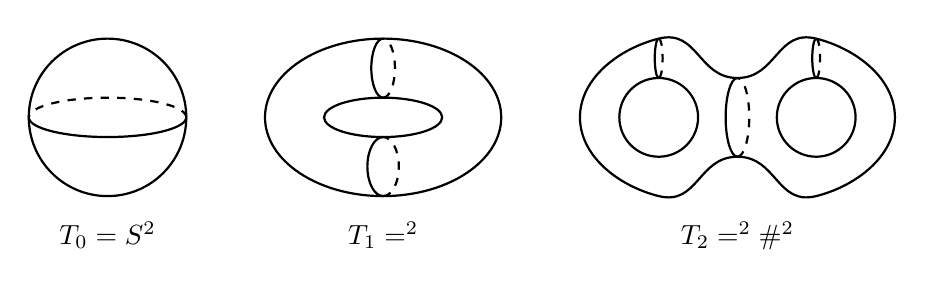
\begin{tikzpicture}
        % Sphère
        \draw[thick] (0,0) circle (1cm);
        \draw[thick] (-1,0) arc (180:360:1 and .25);
        \draw[thick,dashed] (1,0) arc (0:180:1 and .25);
        \node at (0,-1.2) [below] {$T_0=\mathbb S^2$};

        % Tore 
        \draw[thick] (3.5,0) ellipse (1.5cm and 1cm);
        \draw[thick] (3.5,0) ellipse (.75cm and .25cm);
        \draw[thick] (3.5,-1) arc (270:90:.2 and .375);
        \draw[thick,dashed] (3.5,-1) arc (-90:90:.2 and .375);
        \draw[thick] (3.5,.25) arc (270:90:.15 and .375);
        \draw[thick,dashed] (3.5,.25) arc (-90:90:.15 and .375);
        \node at (3.5,-1.2) [below] {$T_1=\T^2$};

        % Quadruble tore
        \node (p1) at (6,0) {};
        \node (p2) at (7,1) {};
        \node (p3) at (8,.5) {};
        \node (p4) at (9,1) {};
        \node (p5) at (10,0) {};
        \node (p6) at (9,-1) {};
        \node (p7) at (8,-.5) {};
        \node (p8) at (7,-1) {};
        \draw[thick] (7,0) circle (.5);
        \draw[thick] (9,0) circle (.5);
        \draw[thick] (8,-.5) arc (270:90:.15 and .5);
        \draw[thick,dashed] (8,-.5) arc (-90:90:.15 and .5);
        \draw[thick] (7,.5) arc (270:90:.05 and .25);
        \draw[thick,dashed] (7,.5) arc (-90:90:.05 and .25);
        \draw[thick] (9,.5) arc (270:90:.05 and .25);
        \draw[thick,dashed] (9,.5) arc (-90:90:.05 and .25);
        \path[thick,draw] plot [smooth cycle,tension=.9] coordinates {(p1) (p2) (p3) (p4) (p5) (p6) (p7) (p8)};
        \node at (8,-1.2) [below] {$T_2=\T^2\#\T^2$};
    \end{tikzpicture}
\end{document}